\section{ISISDLM::Cube\-Io\-Policy$<$ T, TYPEID, IOPolicy $>$ Class Template Reference}
\label{classISISDLM_1_1CubeIoPolicy}\index{ISISDLM::CubeIoPolicy@{ISISDLM::CubeIoPolicy}}
{\tt \#include $<$Cube\-Io\-Policy.h$>$}

Inheritance diagram for ISISDLM::Cube\-Io\-Policy$<$ T, TYPEID, IOPolicy $>$:\begin{figure}[H]
\begin{center}
\leavevmode
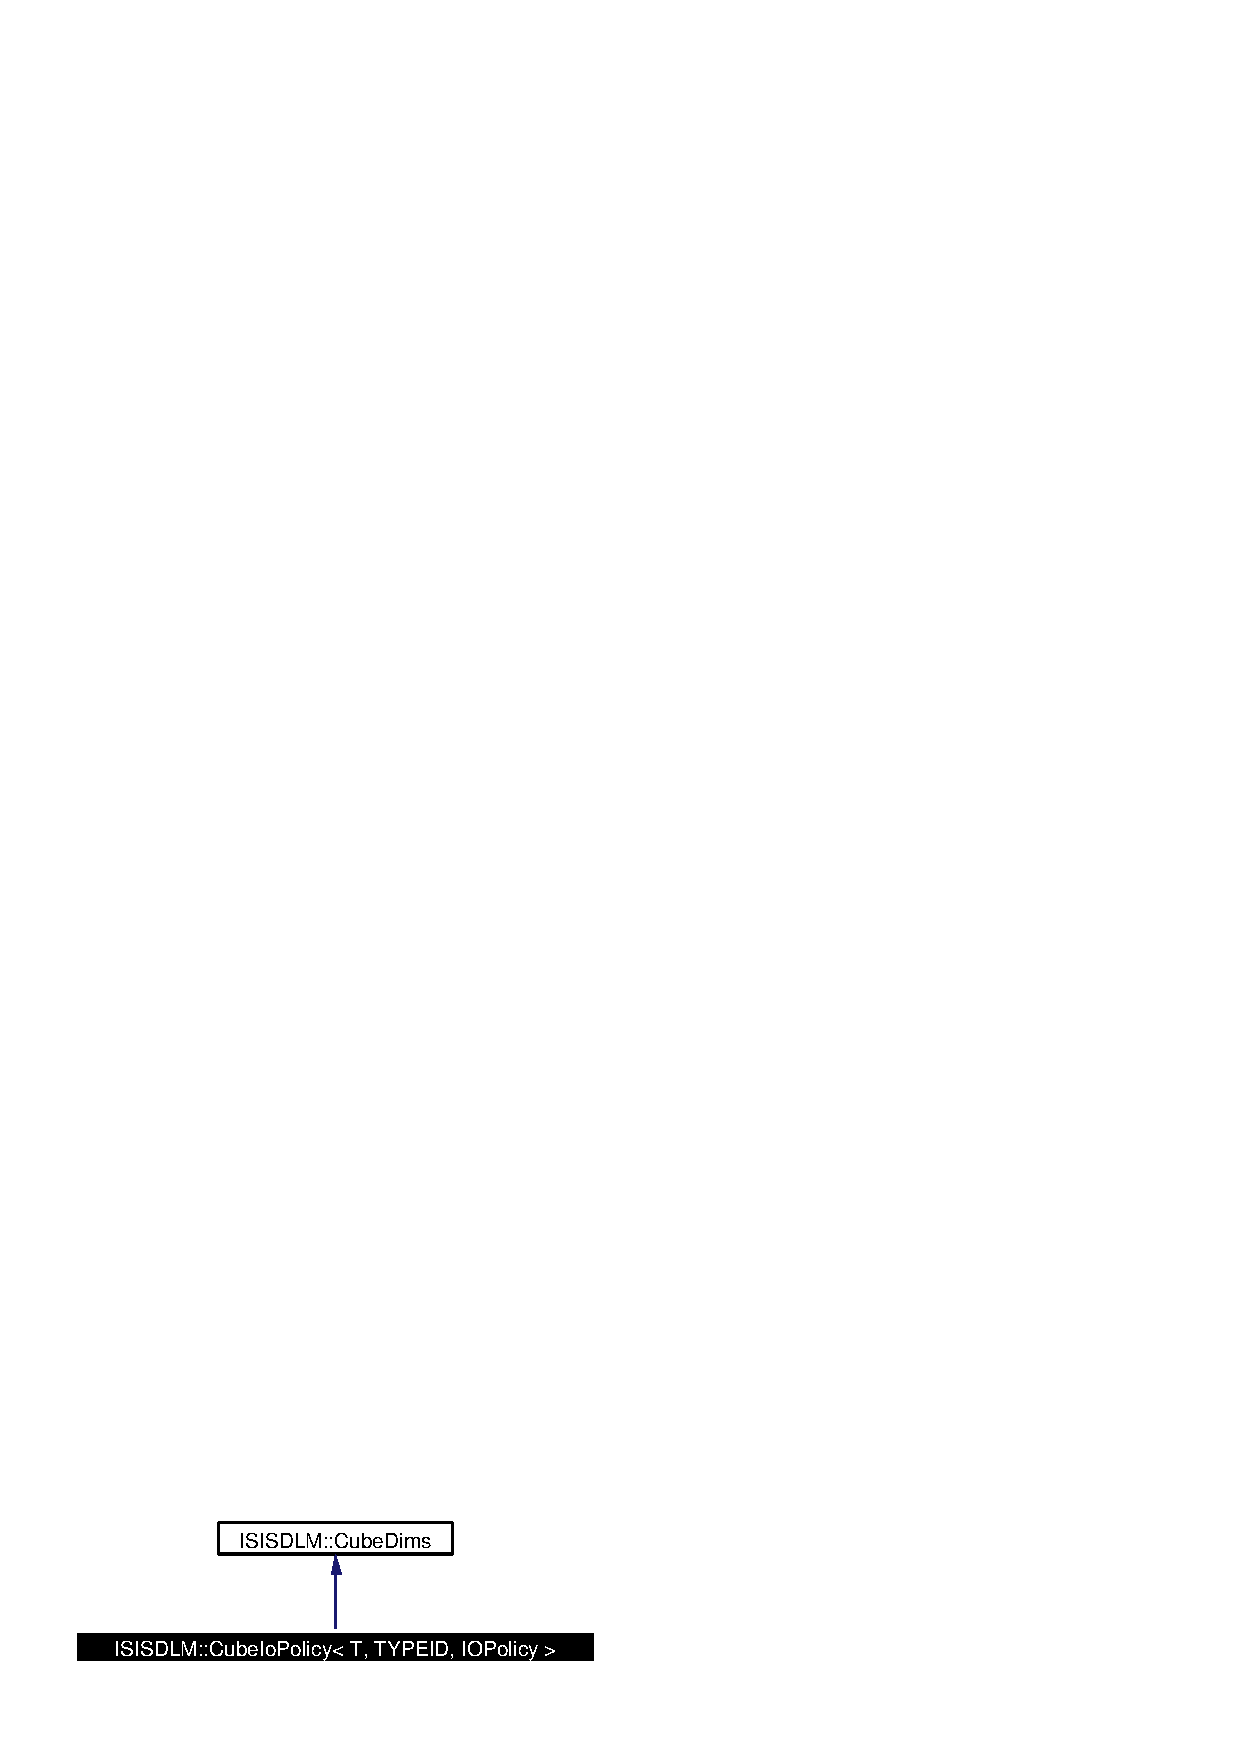
\includegraphics[width=143pt]{classISISDLM_1_1CubeIoPolicy__inherit__graph}
\end{center}
\end{figure}
Collaboration diagram for ISISDLM::Cube\-Io\-Policy$<$ T, TYPEID, IOPolicy $>$:\begin{figure}[H]
\begin{center}
\leavevmode
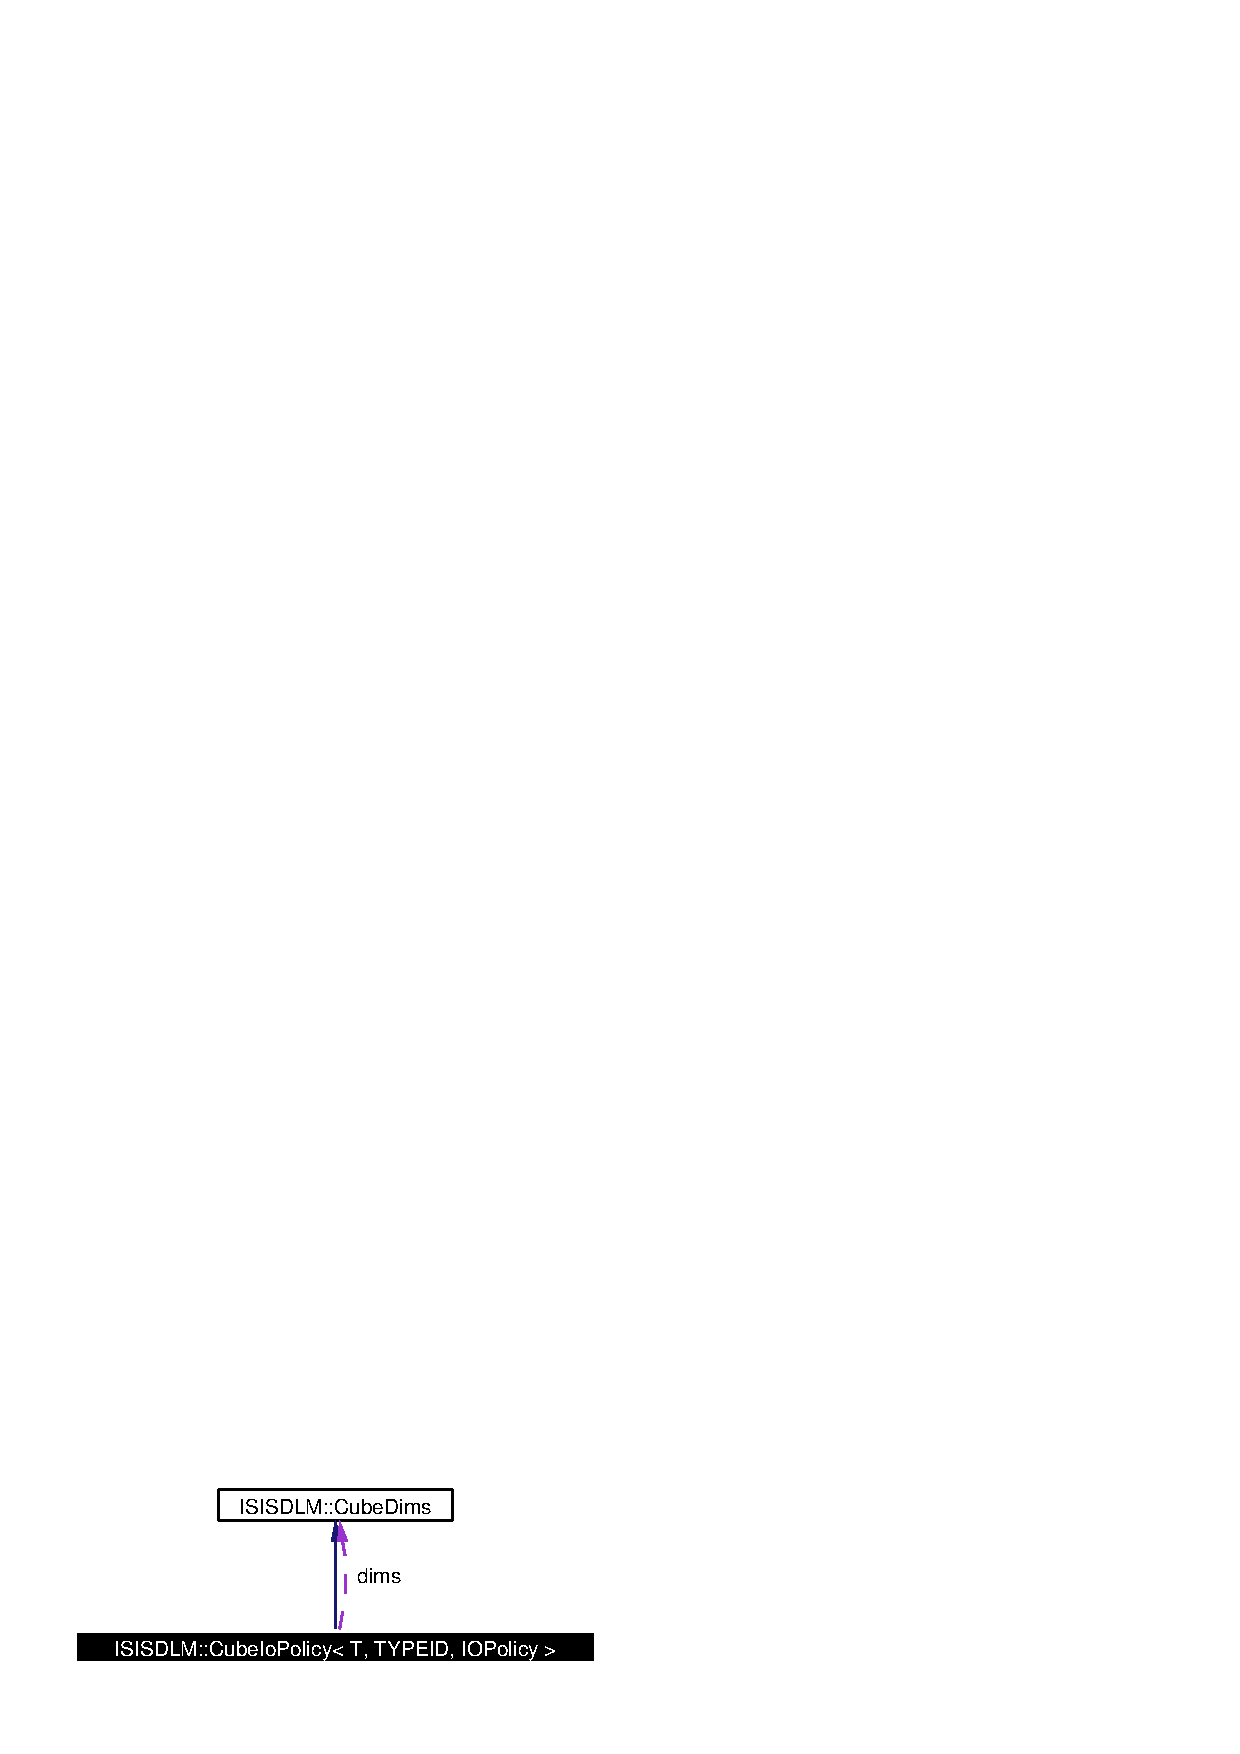
\includegraphics[width=143pt]{classISISDLM_1_1CubeIoPolicy__coll__graph}
\end{center}
\end{figure}
\subsection*{Public Types}
\begin{CompactItemize}
\item 
typedef T {\bf Data\-Type}
\end{CompactItemize}
\subsection*{Public Member Functions}
\begin{CompactItemize}
\item 
{\bf Cube\-Io\-Policy} ()
\item 
{\bf Cube\-Io\-Policy} (const {\bf Cube\-Dims} \&d)
\item 
virtual {\bf $\sim$Cube\-Io\-Policy} ()
\item 
int {\bf get\-Var\-Type} () const
\item 
void {\bf Read} (Isis::Cube \&cube, TNT::Array3D$<$ T $>$ \&data)
\item 
void {\bf Write} (TNT::Array3D$<$ T $>$ \&data, Isis::Cube \&cube)
\end{CompactItemize}
\subsection*{Private Attributes}
\begin{CompactItemize}
\item 
{\bf Cube\-Dims} {\bf dims}
\begin{CompactList}\small\item\em Cube dimensions. \item\end{CompactList}\end{CompactItemize}


\subsection{Detailed Description}
\subsubsection*{template$<$class T, int TYPEID, template$<$ class $>$ class IOPolicy$>$ class ISISDLM::Cube\-Io\-Policy$<$ T, TYPEID, IOPolicy $>$}

Specification reading and writing of data to and from ISIS cubes The {\em {\bf Cube\-Io\-Policy}\/} class handles reading and writing of cube data as specified by the caller. 



\subsection{Member Typedef Documentation}
\index{ISISDLM::CubeIoPolicy@{ISISDLM::Cube\-Io\-Policy}!DataType@{DataType}}
\index{DataType@{DataType}!ISISDLM::CubeIoPolicy@{ISISDLM::Cube\-Io\-Policy}}
\subsubsection{\setlength{\rightskip}{0pt plus 5cm}template$<$class T, int TYPEID, template$<$ class $>$ class IOPolicy$>$ typedef T {\bf ISISDLM::Cube\-Io\-Policy}$<$ T, TYPEID, IOPolicy $>$::{\bf Data\-Type}}\label{classISISDLM_1_1CubeIoPolicy_w0}




\subsection{Constructor \& Destructor Documentation}
\index{ISISDLM::CubeIoPolicy@{ISISDLM::Cube\-Io\-Policy}!CubeIoPolicy@{CubeIoPolicy}}
\index{CubeIoPolicy@{CubeIoPolicy}!ISISDLM::CubeIoPolicy@{ISISDLM::Cube\-Io\-Policy}}
\subsubsection{\setlength{\rightskip}{0pt plus 5cm}template$<$class T, int TYPEID, template$<$ class $>$ class IOPolicy$>$ {\bf ISISDLM::Cube\-Io\-Policy}$<$ T, TYPEID, IOPolicy $>$::{\bf Cube\-Io\-Policy} ()\hspace{0.3cm}{\tt  [inline]}}\label{classISISDLM_1_1CubeIoPolicy_a0}


\index{ISISDLM::CubeIoPolicy@{ISISDLM::Cube\-Io\-Policy}!CubeIoPolicy@{CubeIoPolicy}}
\index{CubeIoPolicy@{CubeIoPolicy}!ISISDLM::CubeIoPolicy@{ISISDLM::Cube\-Io\-Policy}}
\subsubsection{\setlength{\rightskip}{0pt plus 5cm}template$<$class T, int TYPEID, template$<$ class $>$ class IOPolicy$>$ {\bf ISISDLM::Cube\-Io\-Policy}$<$ T, TYPEID, IOPolicy $>$::{\bf Cube\-Io\-Policy} (const {\bf Cube\-Dims} \& {\em d})\hspace{0.3cm}{\tt  [inline]}}\label{classISISDLM_1_1CubeIoPolicy_a1}


\index{ISISDLM::CubeIoPolicy@{ISISDLM::Cube\-Io\-Policy}!~CubeIoPolicy@{$\sim$CubeIoPolicy}}
\index{~CubeIoPolicy@{$\sim$CubeIoPolicy}!ISISDLM::CubeIoPolicy@{ISISDLM::Cube\-Io\-Policy}}
\subsubsection{\setlength{\rightskip}{0pt plus 5cm}template$<$class T, int TYPEID, template$<$ class $>$ class IOPolicy$>$ virtual {\bf ISISDLM::Cube\-Io\-Policy}$<$ T, TYPEID, IOPolicy $>$::$\sim${\bf Cube\-Io\-Policy} ()\hspace{0.3cm}{\tt  [inline, virtual]}}\label{classISISDLM_1_1CubeIoPolicy_a2}




\subsection{Member Function Documentation}
\index{ISISDLM::CubeIoPolicy@{ISISDLM::Cube\-Io\-Policy}!getVarType@{getVarType}}
\index{getVarType@{getVarType}!ISISDLM::CubeIoPolicy@{ISISDLM::Cube\-Io\-Policy}}
\subsubsection{\setlength{\rightskip}{0pt plus 5cm}template$<$class T, int TYPEID, template$<$ class $>$ class IOPolicy$>$ int {\bf ISISDLM::Cube\-Io\-Policy}$<$ T, TYPEID, IOPolicy $>$::get\-Var\-Type () const\hspace{0.3cm}{\tt  [inline]}}\label{classISISDLM_1_1CubeIoPolicy_a3}


\index{ISISDLM::CubeIoPolicy@{ISISDLM::Cube\-Io\-Policy}!Read@{Read}}
\index{Read@{Read}!ISISDLM::CubeIoPolicy@{ISISDLM::Cube\-Io\-Policy}}
\subsubsection{\setlength{\rightskip}{0pt plus 5cm}template$<$class T, int TYPEID, template$<$ class $>$ class IOPolicy$>$ void {\bf ISISDLM::Cube\-Io\-Policy}$<$ T, TYPEID, IOPolicy $>$::Read (Isis::Cube \& {\em cube}, TNT::Array3D$<$ T $>$ \& {\em data})\hspace{0.3cm}{\tt  [inline]}}\label{classISISDLM_1_1CubeIoPolicy_a4}




Here is the call graph for this function:\begin{figure}[H]
\begin{center}
\leavevmode
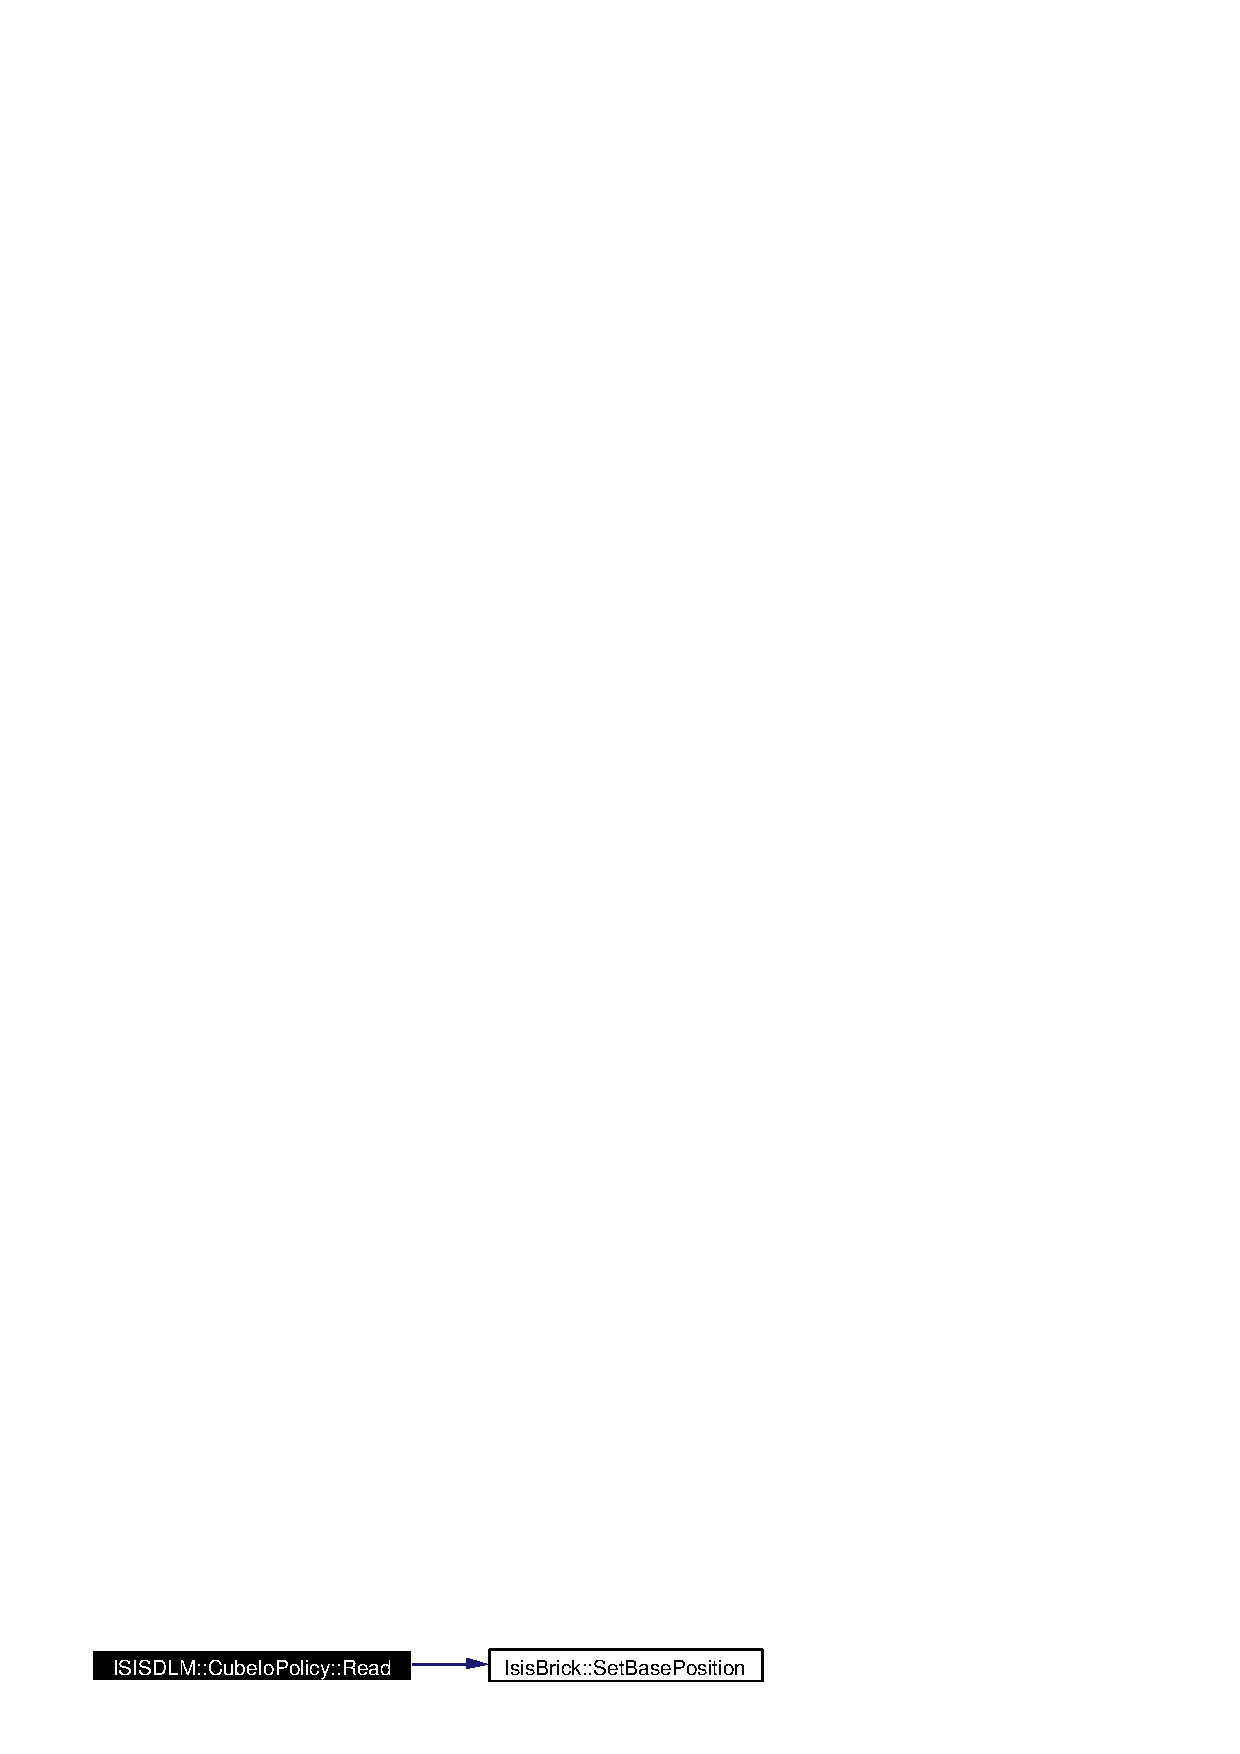
\includegraphics[width=187pt]{classISISDLM_1_1CubeIoPolicy_a4_cgraph}
\end{center}
\end{figure}
\index{ISISDLM::CubeIoPolicy@{ISISDLM::Cube\-Io\-Policy}!Write@{Write}}
\index{Write@{Write}!ISISDLM::CubeIoPolicy@{ISISDLM::Cube\-Io\-Policy}}
\subsubsection{\setlength{\rightskip}{0pt plus 5cm}template$<$class T, int TYPEID, template$<$ class $>$ class IOPolicy$>$ void {\bf ISISDLM::Cube\-Io\-Policy}$<$ T, TYPEID, IOPolicy $>$::Write (TNT::Array3D$<$ T $>$ \& {\em data}, Isis::Cube \& {\em cube})\hspace{0.3cm}{\tt  [inline]}}\label{classISISDLM_1_1CubeIoPolicy_a5}




Here is the call graph for this function:\begin{figure}[H]
\begin{center}
\leavevmode
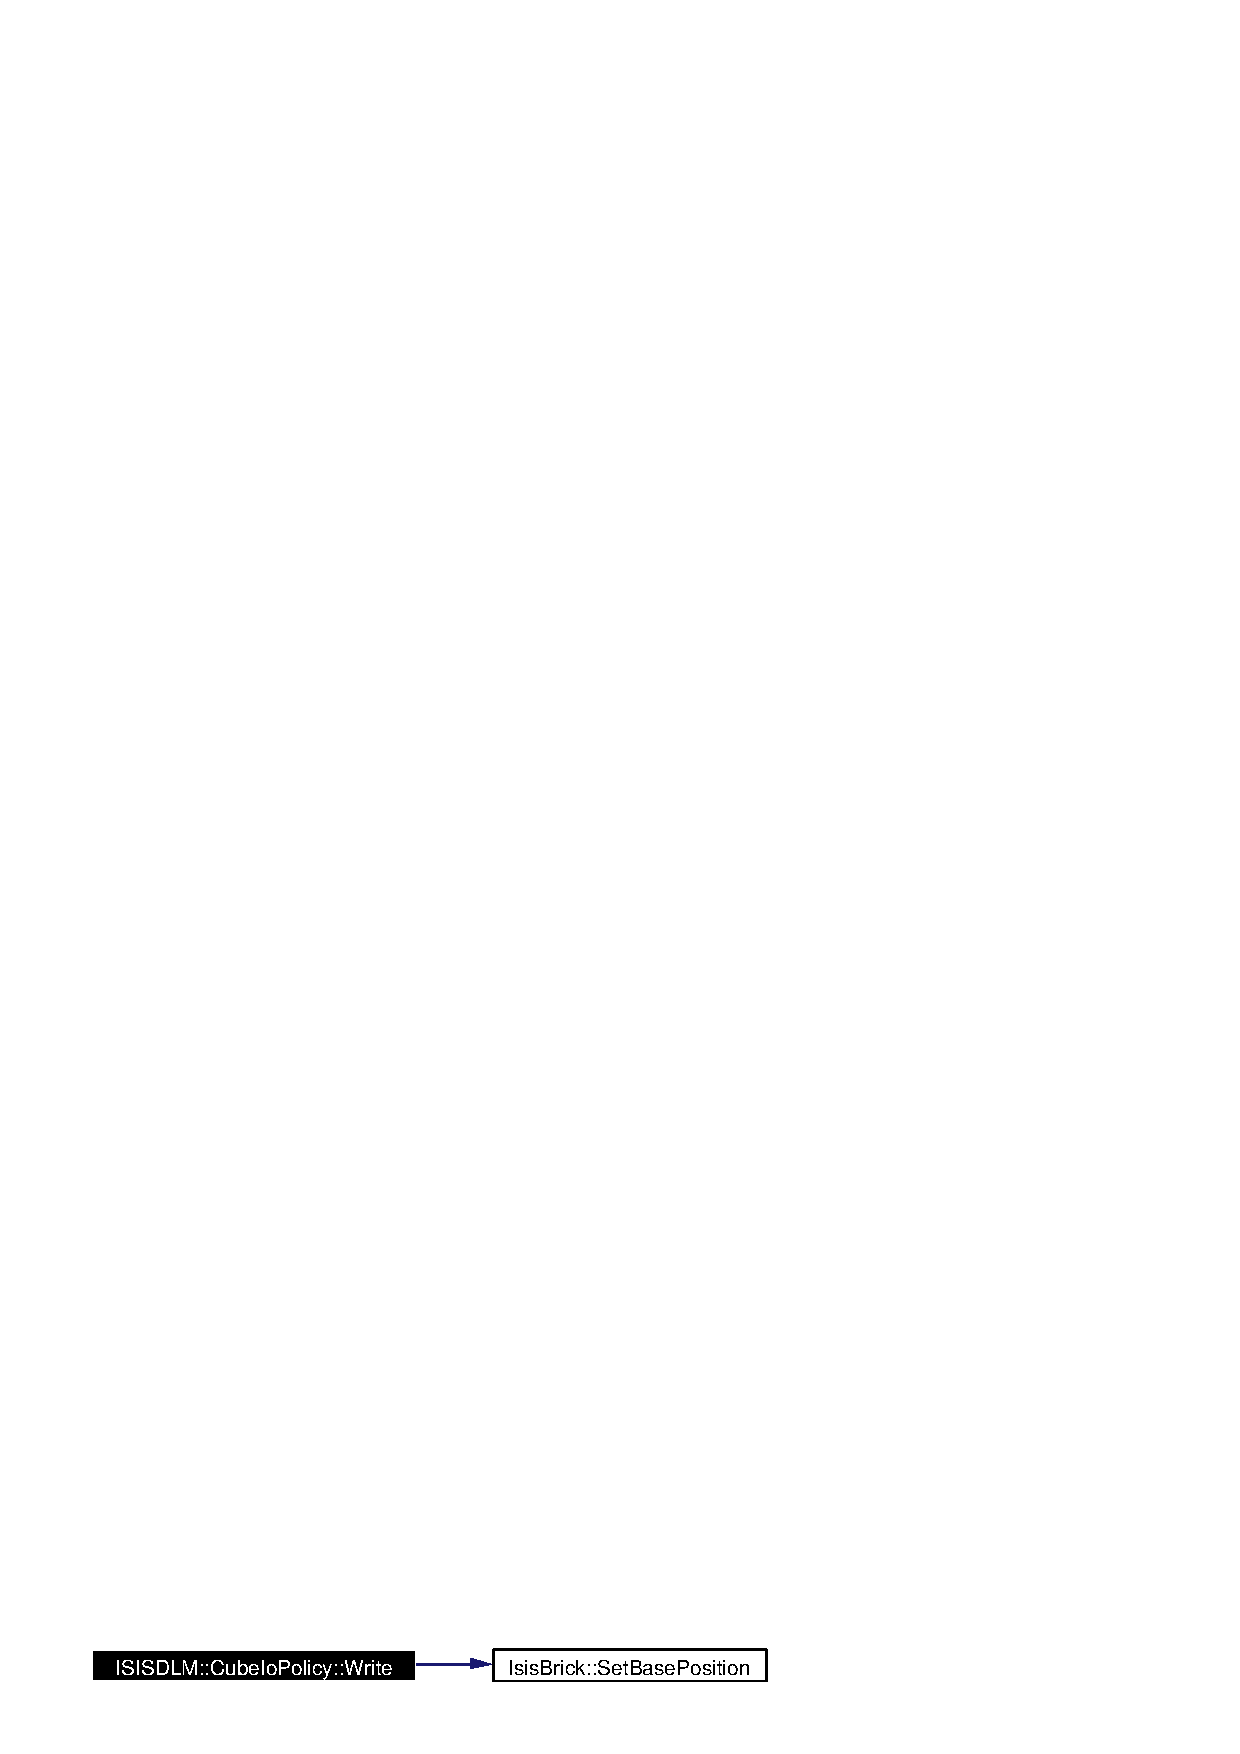
\includegraphics[width=188pt]{classISISDLM_1_1CubeIoPolicy_a5_cgraph}
\end{center}
\end{figure}


\subsection{Member Data Documentation}
\index{ISISDLM::CubeIoPolicy@{ISISDLM::Cube\-Io\-Policy}!dims@{dims}}
\index{dims@{dims}!ISISDLM::CubeIoPolicy@{ISISDLM::Cube\-Io\-Policy}}
\subsubsection{\setlength{\rightskip}{0pt plus 5cm}template$<$class T, int TYPEID, template$<$ class $>$ class IOPolicy$>$ {\bf Cube\-Dims} {\bf ISISDLM::Cube\-Io\-Policy}$<$ T, TYPEID, IOPolicy $>$::{\bf dims}\hspace{0.3cm}{\tt  [private]}}\label{classISISDLM_1_1CubeIoPolicy_r0}


Cube dimensions. 



The documentation for this class was generated from the following file:\begin{CompactItemize}
\item 
{\bf Cube\-Io\-Policy.h}\end{CompactItemize}
